\documentclass[10pt,a4paper]{article}
\usepackage{amsmath}
\usepackage{textcomp}
\usepackage[a4paper,margin=0.8in]{geometry} 
\usepackage{natbib}
\usepackage{longtable}
\usepackage{graphicx}
\usepackage{appendix}

\bibliographystyle{agsm}

%opening
\title{COS 4807 Assignment 1}
\author{Adriaan Louw (53031377)}

\begin{document}

\maketitle

\tableofcontents

\listoffigures

\listoftables


\section{Abstract}
hello
\section{Introduction}

Human attempts to mathematically predict life expectance is not a new endeavour. \cite{Gompertz} introduced an equation to predict life expectancy, which was modified in \cite{Makeham1860} to create the famous Gompertz$-$Makeham law.


Why use machine learning? find relationships that regression analysis cannot \cite{Chen2017}.

Machine learning is used in medicine \cite{Chen2017}.

life expectancy vs mortality rate?

cohort life expectancy vs period life expectancy (https://ourworldindata.org/life-expectancy-how-is-it-calculated-and-how-should-it-be-interpreted)

\cite{Rajkomar2018} Google uses machine learning to predict in hospital medical events for patients. 

\section{Literature Review}

Forecasting Mortality in Developed Countries Tabeau 2001

\subsection{Life tables}

A life table is a table given for a specific year that contains the probability that a person of a certain age will die in that specific year. Life tables are also called actuarial tables and are used by actuaries in the life insurance industry. Table \ref{LifeTable} is an example of a life table taken from \cite{Arias2007}.



Seminal work \cite{Fergany1971}.

\subsection{?Grossman?}
2017 determinants of health: an economic perspective  ????
1972 The Demand for Health: A Theoretical and Empirical Investigation,

\cite{Grossman2000}

\subsection{Life expectancy projections}

The United Nations use a Bayesian model to predict future life expectancy \citep{Raftery2014}.

Lee Carter method \cite{Shang2011} later extended into the Li-Lee model

Siminal work \cite{Lee1992}

\cite{Bongaarts2005}

\subsection{Determinants of life expectancy}



\subsubsection{Income}

The relationship beteen income and life expectancy has been given a lot of attention in academic circles \citep{Preston1975, Hu2015, Chetty2016, Oeppen2019}. 

\cite{Preston1975} was the first to show the relationship between life expectancy and per capita income. His original curve can be seen in Figure \ref{Preston}. As we can see from Figure \ref{Preston}, for low income countries, life expectancy increases rapidly with per capita income. Whereas in high income countries a small increase in per capita income does not have a large effect on life expectancy.

This relationship has also been shown in more recent studies \citep{Chetty2016,Oeppen2019}. Even though \cite{Shkol2019} found that in Russia the Preston curve is not an accurate predictor of life expectancy. They found that the actual life expectancy should be ``substantially higher'' when comparing to the Preston curve predicted value. 

Studies in first world countries involving mortality rather that life expectancy have also found a relationship with income level \citep{Blakely2004,Kalwij2013,VonGaudecker2007}.

Just 16\% of the increase in life expectancy between 1930s and 1960s could be explained by rising income levels \cite{Preston1975}. Which seems to indicate that a coutries life expectancy is dependant on more than income levels.  



\begin{figure}
\centering
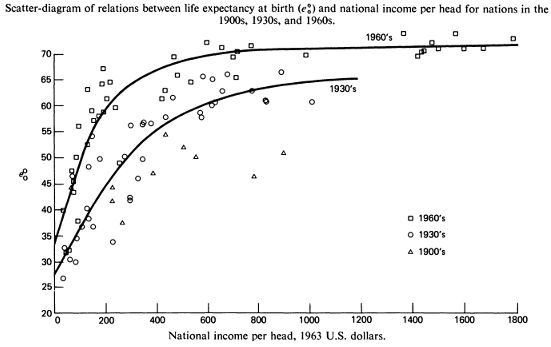
\includegraphics[ height=9cm, width=13cm]{The-original-Preston-Curve-1975.jpg}
\caption{The original Preston curve from \cite{Preston1975}}
\label{Preston}
\end{figure}











\cite{Kalwij2014}

\cite{Oeppen2019} Very Good!!

\cite{Preston1975} is a seminal work according to \cite{Oeppen2019}

inequality \cite{Hu2015}

\cite{Chetty2016} in the US

income inequality does not affect health of a a country \cite{JasonBeckfield2004}

\cite{Tarkiainen2012} (To be downloaded)

\subsubsection{Education atainment}


\cite{Kaplan2015} investigated the relationship between educational atainment and life expectancy in eight states in the United States. They found that even when controlling for variables like income, race, sex and common medical issues like cardiovascular disease, the relationship between educational antainment and life expectance remains statistically significant.

But what is the nature of this correlation? According to \cite{Deary2004} Intelligence Quotient or IQ could explain the association. While \cite{Hayward2015} does not believe in a ``causal relationship'' but rather that it depends on factors like ``time, place, and the social environment''.

In an attempt to find a causal relationship between education and life expectancy, \cite{VanKippersluis2009} investigated the result of the Netherlands increasing the mandatory number of years a child had to attend school to 7 years. It was 6 years previously. \cite{VanKippersluis2009} found a decrease in mortality of 3\% for 81 year old males who had the aditional year of schooling. 


helping individuals to mobilise health resources \cite{Elo1996} from \cite{Deboosere2009}





Study in Belgium \cite{Deboosere2009}


Inverse relationship  \cite{Hoque2019}

netherlands \cite{VanKippersluis2009}

\cite{VanBaal2016a}

\subsubsection{Per capita spending on health}

\cite{Shaw2005} showed that pharmaceutical expenditures shows a positive correlation with life expectancy in OECD countries.

medical spending \cite{Cutler2006}

\subsubsection{Access to safe drinking water}

\subsubsection{Infant mortality}

\cite{CDC1999}

\subsubsection{Turmoil}
\citep{Low2008} p211

\subsection{The gender gap}

\cite{Rochelle2015}

\subsection{Unemployment}
unemployment \cite{Bonamore2015} \cite{Roelfs2011} \cite{Roelfs2015} 

\section{Methodology/Procedure}

There are many studies that attempt to extrapolate future life expectancy for countries based on current data. This includes studies for high income countries \citep{Kontis2017} and low income countries ????{cite}.

This study will attempt to create a model that can predict life expectancy for a country based on various socio-economic conditions in the country.



segment data into groups where each group has the same amount of data points???

Unlike \cite{Shaw2005}, this study will not take into account the age distribution of eacmh country.

As for HDI from \cite{Bulled2010}
Adult literacy rate

primary secondary and tertiary enrolment ratios

GDP per Capita (Purchasing power parity )


The impact of finishing secondary school is different before vs after the seconf world war \cite{Deboosere2009}

\subsection{Choice of dataset}

\subsection{Regression}

\subsection{k-Nearest Neighbour}

\subsection{Support Vector Machines}

\subsection{Cross-validation}

\section{Analysis}

\section{Conclusion}

\section{Recommendations}

\addcontentsline{toc}{section}{References}
\bibliography{mybib}

\appendix
\appendixpage

\begin{longtable}{|c|c|c|c|c|c|c|}
\caption{Life table for the total population: United States, 2003 \citep{Arias2007}}\\
 \hline \\
      &               &              &               &               & Total        &              \\
       & Probability   &              & Number        & Person-years  & number of    &              \\
       & of dying      & Number       & dying         & lived         & person-years & Expectation  \\
       & between       & surviving to & between       & between       & lived above  & of life      \\
       & ages x to x+1 & age x        & ages x to x+1 & ages x to x+1 & age x        & at age x     \\
\hline  \\
Age    & q(x)          & l(x)         & d(x)          & L(x)          & T(x)         & e(x)         \\
\hline \\
0-1    & 0.006865      & 100,000      & 687           & 99,394        & 7,743,016    & 77.4         \\
1-2    & 0.000469      & 99,313       & 47            & 99,290        & 7,643,622    & 77.0         \\
2-3    & 0.000337      & 99,267       & 33            & 99,250        & 7,544,332    & 76.0         \\
3-4    & 0.000254      & 99,233       & 25            & 99,221        & 7,445,082    & 75.0         \\
4-5    & 0.000194      & 99,208       & 19            & 99,199        & 7,345,861    & 74.0         \\
5-6    & 0.000177      & 99,189       & 18            & 99,180        & 7,246,663    & 73.1         \\
6-7    & 0.000160      & 99,171       & 16            & 99,163        & 7,147,482    & 72.1         \\
7-8    & 0.000147      & 99,156       & 15            & 99,148        & 7,048,319    & 71.1         \\
8-9    & 0.000132      & 99,141       & 13            & 99,134        & 6,949,171    & 70.1         \\
9-10   & 0.000117      & 99,128       & 12            & 99,122        & 6,850,036    & 69.1         \\
10-11  & 0.000109      & 99,116       & 11            & 99,111        & 6,750,914    & 68.1         \\
11-12  & 0.000118      & 99,105       & 12            & 99,100        & 6,651,803    & 67.1         \\
12-13  & 0.000157      & 99,094       & 16            & 99,086        & 6,552,704    & 66.1         \\
13-14  & 0.000233      & 99,078       & 23            & 99,067        & 6,453,618    & 65.1         \\
14-15  & 0.000339      & 99,055       & 34            & 99,038        & 6,354,551    & 64.2         \\
15-16  & 0.000460      & 99,022       & 46            & 98,999        & 6,255,513    & 63.2         \\
16-17  & 0.000577      & 98,976       & 57            & 98,947        & 6,156,514    & 62.2         \\
17-18  & 0.000684      & 98,919       & 68            & 98,885        & 6,057,566    & 61.2         \\
18-19  & 0.000769      & 98,851       & 76            & 98,813        & 5,958,681    & 60.3         \\
19-20  & 0.000832      & 98,775       & 82            & 98,734        & 5,859,868    & 59.3         \\
20-21  & 0.000894      & 98,693       & 88            & 98,649        & 5,761,134    & 58.4         \\
21-22  & 0.000954      & 98,605       & 94            & 98,558        & 5,662,485    & 57.4         \\
22-23  & 0.000990      & 98,511       & 98            & 98,462        & 5,563,928    & 56.5         \\
23-24  & 0.000997      & 98,413       & 98            & 98,364        & 5,465,466    & 55.5         \\
24-25  & 0.000982      & 98,315       & 97            & 98,267        & 5,367,101    & 54.6         \\
25-26  & 0.000960      & 98,219       & 94            & 98,171        & 5,268,835    & 53.6         \\
26-27  & 0.000942      & 98,124       & 92            & 98,078        & 5,170,663    & 52.7         \\
27-28  & 0.000936      & 98,032       & 92            & 97,986        & 5,072,585    & 51.7         \\
28-29  & 0.000947      & 97,940       & 93            & 97,894        & 4,974,599    & 50.8         \\
29-30  & 0.000974      & 97,847       & 95            & 97,800        & 4,876,705    & 49.8         \\
30-31  & 0.001008      & 97,752       & 98            & 97,703        & 4,778,906    & 48.9         \\
31-32  & 0.001046      & 97,654       & 102           & 97,603        & 4,681,203    & 47.9         \\
32-33  & 0.001097      & 97,551       & 107           & 97,498        & 4,583,600    & 47.0         \\
33-34  & 0.001162      & 97,444       & 113           & 97,388        & 4,486,102    & 46.0         \\
34-35  & 0.001244      & 97,331       & 121           & 97,271        & 4,388,715    & 45.1         \\
35-36  & 0.001336      & 97,210       & 130           & 97,145        & 4,291,444    & 44.1         \\
36-37  & 0.001441      & 97,080       & 140           & 97,010        & 4,194,299    & 43.2         \\
37-38  & 0.001567      & 96,940       & 152           & 96,864        & 4,097,289    & 42.3         \\
38-39  & 0.001714      & 96,788       & 166           & 96,705        & 4,000,424    & 41.3         \\
39-40  & 0.001874      & 96,623       & 181           & 96,532        & 3,903,719    & 40.4         \\
40-41  & 0.002038      & 96,442       & 197           & 96,343        & 3,807,187    & 39.5         \\
41-42  & 0.002207      & 96,245       & 212           & 96,139        & 3,710,844    & 38.6         \\
42-43  & 0.002389      & 96,033       & 229           & 95,918        & 3,614,705    & 37.6         \\
43-44  & 0.002593      & 95,803       & 248           & 95,679        & 3,518,787    & 36.7         \\
44-45  & 0.002819      & 95,555       & 269           & 95,420        & 3,423,108    & 35.8         \\
45-46  & 0.003064      & 95,285       & 292           & 95,139        & 3,327,688    & 34.9         \\
46-47  & 0.003322      & 94,993       & 316           & 94,836        & 3,232,548    & 34.0         \\
47-48  & 0.003589      & 94,678       & 340           & 94,508        & 3,137,713    & 33.1         \\
48-49  & 0.003863      & 94,338       & 364           & 94,156        & 3,043,205    & 32.3         \\
49-50  & 0.004148      & 93,974       & 390           & 93,779        & 2,949,049    & 31.4         \\
50-51  & 0.004458      & 93,584       & 417           & 93,375        & 2,855,270    & 30.5         \\
51-52  & 0.004800      & 93,167       & 447           & 92,943        & 2,761,895    & 29.6         \\
52-53  & 0.005165      & 92,719       & 479           & 92,480        & 2,668,952    & 28.8         \\
53-54  & 0.005554      & 92,241       & 512           & 91,984        & 2,576,472    & 27.9         \\
54-55  & 0.005971      & 91,728       & 548           & 91,454        & 2,484,487    & 27.1         \\
55-56  & 0.006423      & 91,181       & 586           & 90,888        & 2,393,033    & 26.2         \\
56-57  & 0.006925      & 90,595       & 627           & 90,281        & 2,302,145    & 25.4         \\
57-58  & 0.007496      & 89,968       & 674           & 89,630        & 2,211,864    & 24.6         \\
58-59  & 0.008160      & 89,293       & 729           & 88,929        & 2,122,234    & 23.8         \\
59-60  & 0.008927      & 88,565       & 791           & 88,169        & 2,033,305    & 23.0         \\
60-61  & 0.009827      & 87,774       & 863           & 87,343        & 1,945,136    & 22.2         \\
61-62  & 0.010831      & 86,911       & 941           & 86,441        & 1,857,793    & 21.4         \\
62-63  & 0.011872      & 85,970       & 1021          & 85,460        & 1,771,352    & 20.6         \\
63-64  & 0.012891      & 84,949       & 1095          & 84,402        & 1,685,892    & 19.8         \\
64-65  & 0.013908      & 83,854       & 1166          & 83,271        & 1,601,490    & 19.1         \\
65-66  & 0.015003      & 82,688       & 1241          & 82,068        & 1,518,219    & 18.4         \\
66-67  & 0.016267      & 81,448       & 1325          & 80,785        & 1,436,151    & 17.6         \\
67-68  & 0.017699      & 80,123       & 1418          & 79,414        & 1,355,366    & 16.9         \\
68-69  & 0.019320      & 78,705       & 1521          & 77,944        & 1,275,953    & 16.2         \\
69-70  & 0.021108      & 77,184       & 1629          & 76,369        & 1,198,008    & 15.5         \\
70-71  & 0.022950      & 75,555       & 1734          & 74,688        & 1,121,639    & 14.8         \\
71-72  & 0.024904      & 73,821       & 1838          & 72,902        & 1,046,951    & 14.2         \\
72-73  & 0.027151      & 71,982       & 1954          & 71,005        & 974,050      & 13.5         \\
73-74  & 0.029784      & 70,028       & 2086          & 68,985        & 903,044      & 12.9         \\
74-75  & 0.032753      & 67,942       & 2225          & 66,830        & 834,059      & 12.3         \\
75-76  & 0.035831      & 65,717       & 2355          & 64,540        & 767,230      & 11.7         \\
76-77  & 0.038987      & 63,362       & 2470          & 62,127        & 702,690      & 11.1         \\
77-78  & 0.042503      & 60,892       & 2588          & 59,598        & 640,563      & 10.5         \\
78-79  & 0.046557      & 58,304       & 2714          & 56,947        & 580,965      & 10.0         \\
79-80  & 0.051200      & 55,589       & 2846          & 54,166        & 524,019      & 9.4          \\
80-81  & 0.056335      & 52,743       & 2971          & 51,258        & 469,853      & 8.9          \\
81-82  & 0.061837      & 49,772       & 3078          & 48,233        & 418,595      & 8.4          \\
82-83  & 0.067856      & 46,694       & 3168          & 45,110        & 370,362      & 7.9          \\
83-84  & 0.074504      & 43,526       & 3243          & 41,904        & 325,252      & 7.5          \\
84-85  & 0.081975      & 40,283       & 3302          & 38,632        & 283,348      & 7.0          \\
85-86  & 0.089682      & 36,981       & 3317          & 35,322        & 244,716      & 6.6          \\
86-87  & 0.098031      & 33,664       & 3300          & 32,014        & 209,394      & 6.2          \\
87-88  & 0.107059      & 30,364       & 3251          & 28,739        & 177,380      & 5.8          \\
88-89  & 0.116804      & 27,113       & 3167          & 25,530        & 148,641      & 5.5          \\
89-90  & 0.127300      & 23,946       & 3048          & 22,422        & 123,111      & 5.1          \\
90-91  & 0.138581      & 20,898       & 2896          & 19,450        & 100,689      & 4.8          \\
91-92  & 0.150676      & 18,002       & 2712          & 16,646        & 81,239       & 4.5          \\
92-93  & 0.163611      & 15,289       & 2502          & 14,039        & 64,594       & 4.2          \\
93-94  & 0.177408      & 12,788       & 2269          & 11,654        & 50,555       & 4.0          \\
94-95  & 0.192080      & 10,519       & 2021          & 9,509         & 38,901       & 3.7          \\
95-96  & 0.207636      & 8,499        & 1765          & 7,616         & 29,392       & 3.5          \\
96-97  & 0.224075      & 6,734        & 1509          & 5,980         & 21,776       & 3.2          \\
97-98  & 0.241387      & 5,225        & 1261          & 4,594         & 15,796       & 3.0          \\
98-99  & 0.259552      & 3,964        & 1029          & 3,449         & 11,202       & 2.8          \\
99-100 & 0.278539      & 2,935        & 818           & 2,526         & 7,752        & 2.6          \\
100+   & 1.00000       & 2,118        & 2118          & 5,226         & 5,226        & 2.5          
\hline 
\label{LifeTable}
\end{longtable}

\addappheadtotoc



\end{document}
